\documentclass[10pt]{article}
\usepackage{NotesTeX} %/Path/to/package should be replaced with package location
\usepackage{lipsum}
\usepackage{tensor}
\usepackage{graphicx,wrapfig,float,slashed,subcaption,bbold,bm}
\usepackage{amsmath,mathtools,amssymb,epsfig,graphicx,xcolor}
\usepackage{epstopdf}
\epstopdfsetup{update}
\usepackage{ragged2e}
\usepackage{mciteplus}
\usepackage[many]{tcolorbox}
\usepackage{pgfplots}
\pgfplotsset{compat=1.5.1}
\usepackage{tikz}
\usetikzlibrary{babel}
\tikzset{>=latex}
\usepackage{hyperref}

\newcommand{\bs}{\textbackslash}
\newcommand{\nc}{\newcommand}
\newcommand{\non}{\nonumber}	
\newcommand{\noi}{\noindent}
\newcommand{\barx}{\bar{x}}
%

\newcommand{\hsp}{\hspace{0.5cm}}
\newcommand{\lsp}{\hspace{1cm}}
\newcommand{\Lsp}{\hspace{2cm}}
%\nnewcommand{\LLsp}{\lsp\lsp}
\newcommand{\lra}{\longrightarrow}
\newcommand{\p}{\prime}
\newcommand{\sgn}{\text{sgn}}
\newcommand{\ph}{\varphi}


\newcommand{\beq}{\begin{equation}}  \newcommand{\eeq}{\end{equation}}
\newcommand{\bea}{\begin{eqnarray}}  \newcommand{\eea}{\end{eqnarray}}
\newcommand{\baa}{\begin{array}}     \newcommand{\eaa}{\end{array}}
\newcommand{\bit}{\begin{itemize}}   \newcommand{\eit}{\end{itemize}}
\newcommand{\ben}{\begin{enumerate}} \newcommand{\een}{\end{enumerate}}
\newcommand{\bce}{\begin{center}}    \newcommand{\ece}{\end{center}}
\newcommand{\bpm}{\begin{pmatrix}}   \newcommand{\epm}{\end{pmatrix}}
\newcommand{\bvt}{\begin{verbatim}}  
\newcommand{\evt}{\end{verbatim}}
\title{{\Huge General Relativity}\\{\Large{Class 14}}} %replace with class number
\author{Aditya Mewar}
\emailAdd{am1993@utexas.edu} %replace with your email
\begin{document}
	\maketitle
	\flushbottom
	\newpage
	\pagestyle{fancynotes}
    
\part{First Look at Black Holes}
%\section{Recap}
So far we have sufficiently developed our mathematical toolbox to begin to analyze the physics around certain black holes. We will begin by analyzing external(outside of gravitational body) spherically symmetric vaccum solution of Einsteins equation which is given by a particular metric described below. 

\section{The Schwarzchild Solution} \label{sec:rev_dual_vectors}
The line element outside a spherically symmetric black hole is: 
\begin{equation}
 ds^2 =- (1 -\frac{2GM}{r})dt^2 + (1-\frac{2GM}{r})^{-1} dr^2 + r^2 d\Omega^2
 \label{eq:metric}
\end{equation}


We will accept this as the metric without derivation at the time being. $M$ is interpreted as the black hole mass, and $d\Omega^2 = d\theta^2 + \sin^2{\theta}d\phi^2$. In tensor form this is represented as: 

\begin{equation}
g_{\mu\nu} = \begin{bmatrix}
       - (1 -\frac{2GM}{r})   & 0 & 0 &0 \\
   0     &  (1-\frac{2GM}{r})^{-1} &0 & 0 \\
   0&0&r^2&0\\
    0   & 0 & 0 & r^2 \sin^2{\theta} \\
\end{bmatrix}
\end{equation}

The parameters can take the range:

\begin{equation}
t \in (-\infty,\infty),
\theta \in (-\pi,\pi),
\phi \in (0,2\pi),
r  \in (2M, \infty)
\end{equation}

So far these parameters dont necessarily correspond to physical coordinates so we will have to explore the metric to identify them. Let us first see if there are symmetries of the metric. We see that $t,\phi$ do not appear in $g_{\mu\nu}$. This further implies spherical symmetry. We can also see that as $r \rightarrow \infty$ then, 

\begin{equation}
ds^2 = -dt^2 + dr^2 +r^2d\Omega^2
\end{equation}

This is the line element in spherical polar coordinates in flat space. We will now try to give physical meaning to coordinates by looking at invariant quantities such as proper distance and time. We must express the physical nature of these parameters this way because arbitrary metrics can describe the same situation. 

\section{Radial Coordinate} 

Let us begin by considering a proper length in this metric. 

\begin{equation}
S = \int \sqrt{g_{\mu\nu} \frac{dx^\mu}{d\lambda} \frac{dx^\nu}{d\lambda} } d\lambda
\end{equation}

And further we will assume that $r=t=constant$, $\theta = \frac{\pi}{2}$,$ \phi = \lambda$. This gives $\frac{dx^\mu}{d\lambda} = [0,0,0,1]$.Then, 

\begin{equation}
S =\int \sqrt{g_{\mu\nu}} d\lambda = \int \sqrt{r^2\sin^2(\frac{\pi}{2})} d\lambda = r \int_{0}^{2\pi} d\lambda = 2 \pi r
\end{equation}

This result implies that $r$ can be interpreted as the radius of a circle, or "areal radius". This radius is the radius of a spherical shell with the origin as the black hole. We now notice a strange property of the metric by varying $r$ and keeping other coordinates constant. 

\begin{equation}
ds^2 =\frac{dr^2}{1 - \frac{2M}{r}}
\end{equation}


This implies that $ ds > dr $ when $r > 2M$. This actually means that observers standing on concentric shells around the black hole would measure the distance $ds$ between them and find out that the difference is larger than $dr$, the difference in the radii of the sphere around the black hole. This phenomenon is represented in an embedding diagram in spacelike slices. 
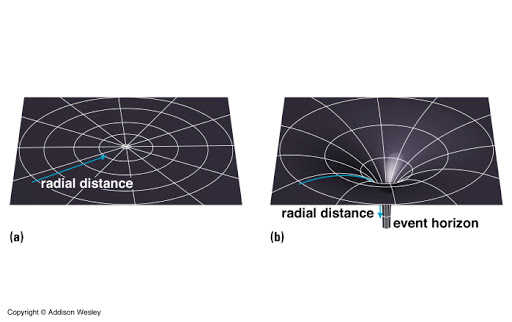
\includegraphics[scale=.5]{Figures/embed.jpg} 
\section{Behavior of light around Black Hole}

We can follow a similar train of logic regarding the time like  coordinate of the metric. Let us consider a timelike slice with $\theta,\phi$ both constants. 

\begin{equation}
ds^2 = d\tau^2 = \sqrt{1-\frac{2M}{r}} dt^2
\end{equation}

Again we see this is smaller than $dt$ meaning that observers near the black hole will experience slower ticking clocks compared to distant observers. This is known as gravitational time dilation. 

Let us now consider the metric when it is null, $ds^2 = 0$.  Let us continue to have $\theta,\phi$ arbitrary but fixed, and let us find an expression for $\frac{dt}{dr}$. 

\begin{equation}
- (1 - \frac{2M}{r})dt^2 + \frac{dr^2}{(1-\frac{2M}{r})} = 0 
\end{equation}

We see that 

\begin{equation}
\frac{dt}{dr} =  \pm \frac{1}{(1-\frac{2M}{r})}
\end{equation}

This relationship indicates that light will slow to zero when nearing the black hole and that it will never be able to escape the black hole. This can be thought of as the light cone closing at it approaches the singularity. 


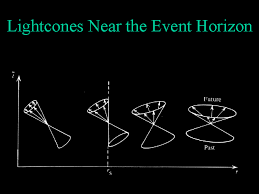
\includegraphics[scale=.5]{Figures/bh.png} 
\section{Behavior of timelike worldlines around the Black Hole}

In order to do calculations we need to assert some relationships that we will prove later. They are, 

\begin{equation}
\frac{E}{m} = \mathcal{E} = (1 - \frac{2M}{r}) \frac{dt}{d\tau} 
\end{equation}

\begin{equation}
\frac{L}{m} = \mathcal{L} = r^2 \frac{d\phi}{d\tau}
\end{equation}


The above equations are implications of the symmetries in $t$ and $\phi$. Specifically, the former implies conservation of energy and the latter conservation of angular momentum and they are both constants. Now lets use the try to identify $\frac{dt}{dr}$ in terms of the line element. Let's begin with the four velocity normalization condition. 

\begin{equation}
\begin{split}
g_{\mu\nu} \frac{dx^\mu}{d\lambda}  \frac{dx^\nu}{d\lambda} = \vec{U} \cdot \vec{U} = -1 \\
=g_{tt}(\frac{\partial{t}}{\partial{\tau}})^2 +g_{rr}(\frac{\partial{r}}{\partial{\tau}})^2 \\
 = (1- \frac{2M}{r})(\frac{\partial{t}}{\partial{\tau}})^2+(\frac{1}{1-\frac{2M}{r}})(\frac{\partial{r}}{\partial{\tau}})^2 
\end{split}
\end{equation}



Now we will use (4.1) to eliminate $\frac{dt}{d\tau}$ and solve for $\frac{dr}{d\tau}$. We get that, 

\begin{equation}
\frac{dr^2}{d\tau^2} = \mathcal{E}^2 - (1-\frac{2M}{r})
\end{equation}

Now we will try identify what an distant observer would see as $\frac{dr}{dt}$ for something falling into a black hole. So if we start at rest then $ E = m$ and $ \mathcal{E} =1$. This readily leads to $\frac{dt}{d\tau} = \frac{1}{(1- \frac{2M}{r})}$.  This leads to, 

\begin{equation}
\frac{dr}{d\tau} = \pm \sqrt{\frac{2M}{r}}
\end{equation}

A distant observer would see: 

\begin{equation}
\begin{split} 
\frac{dr}{dt} = \frac{dr}{d\tau}\frac{d\tau}{dt} =-\sqrt{ \frac{2M}{r}}(1 - \frac{2M}{r})
\end{split}
\end{equation}









\end{document}
